\subsection{Postoperativt}
Udover præoperative faktorer kan der postoperative komplikationer, herunder komplikation påstået under og efter operation, som kan have indflydelse på en længere indlæggelsesvarighed for patienten. Postoperativ estimeres indlæggelsesvarigheden ligeledes ikke på nuværende tidspunkt, hvorfor der er taget udgangspunkt i informationspjecer fra ortopædkirurgisk afdeling på Aalborg Universitetshospital samt studier der påviser dette.

\subsubsection{Komplikation under operation}
Varigheden af operationen 
*** SKRIV NOGET HER** 

\begin{figure}[H]
	%\flushleft 
	\centering
	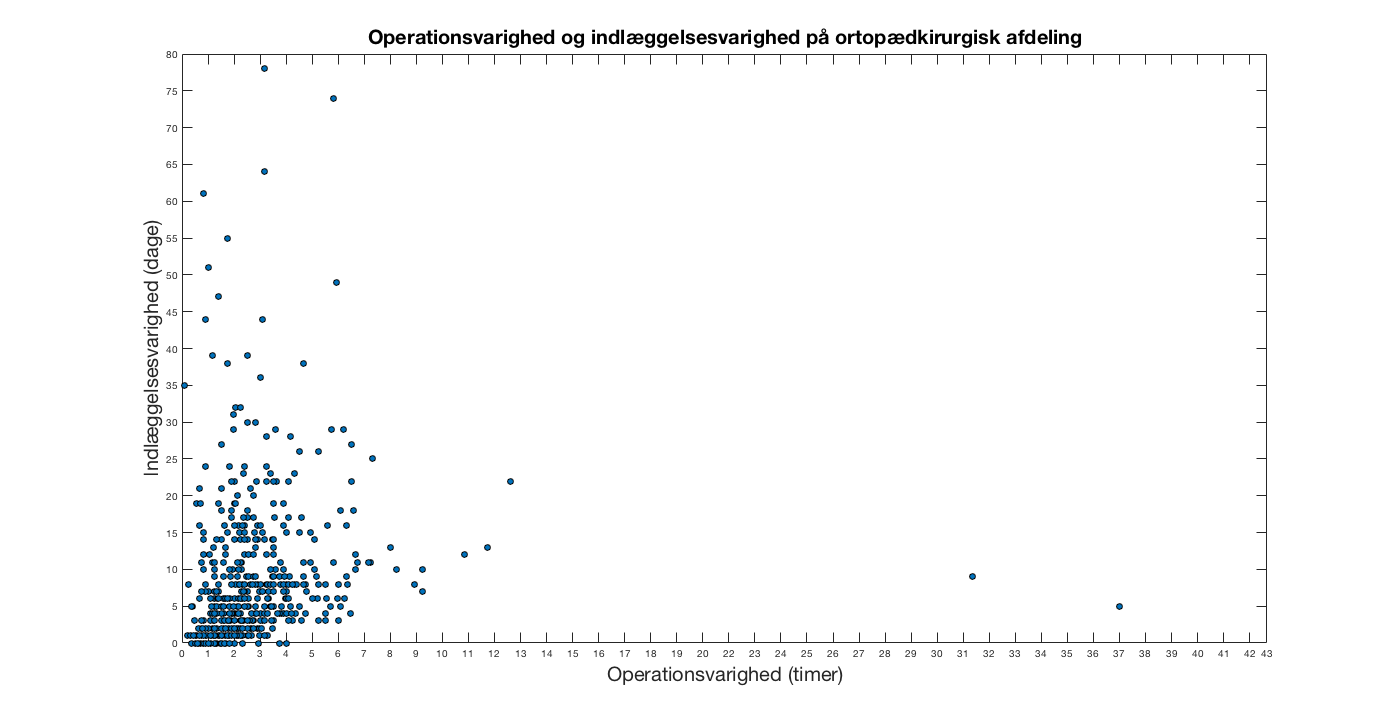
\includegraphics[scale=0.35]{figures/opindlaeg.png}
	%\flushleft
	\caption{\textit{Træning og indlæggelsesvarighed for patienter på ortopædkirurgisk afdeling. Træning er opdelt i ingen træning dagen efter operation og træning dagen efter operation. Dette er over en periode på 3 måneder fra den 1. august til den 31. oktober år 2014.}}
	\label{opindlaeg}
	\end{figure}

\noindent
*** SKRIV NOGET HER ***


\subsubsection{Komplikationer efter operationen}
Det tyder på, at bevægelighed efter operation er vigtigt for, at komme sig hurtigt efter operationen, da dette er med til, at mindske risikoen for komplikationer og smerter efter operationen. Sammenhængen mellem træning og indlæggelsesvarigheden er illustreret på \figref{traeningindlaeg}.

\begin{figure}[H]
	%\flushleft 
	\centering
	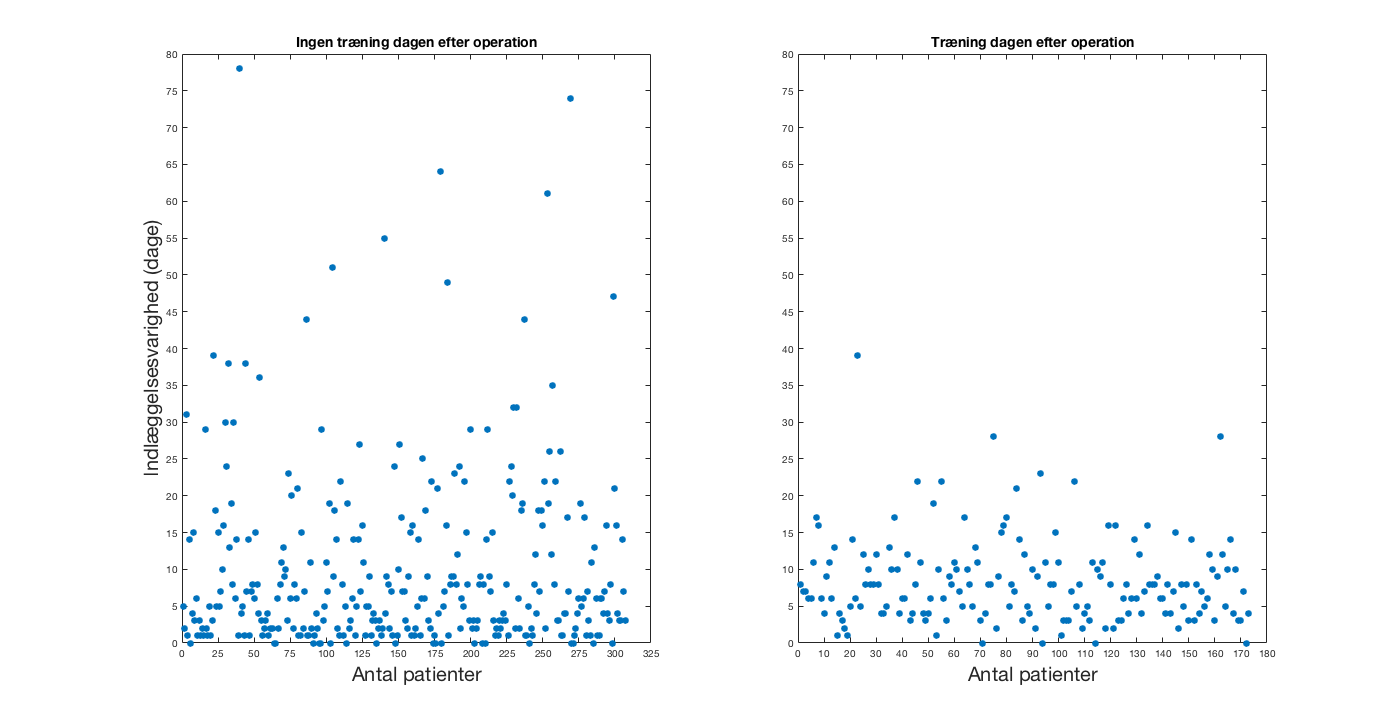
\includegraphics[scale=0.35]{figures/traeningindlaeg.png}
	%\flushleft
	\caption{\textit{Træning og indlæggelsesvarighed for patienter på ortopædkirurgisk afdeling. Træning er opdelt i ingen træning dagen efter operation og træning dagen efter operation. Dette er over en periode på 3 måneder fra den 1. august til den 31. oktober år 2014.}}
	\label{traeningindlaeg}
	\end{figure}

\noindent
På \figref{traeningindlaeg} fremgår det, at der er flere patienter  der ikke træner dagen efter operationen. Ligeledes er variationen i indlæggelsesvarighed større for patienter der ikke træner dagen efter end patienter der træner. Den gennemsnitlige indlæggelsesvarighed for patienter, der ikke træner dagen efter operation er 10 dage. Modsat er patienter, som træner dagen efter operationen 8,2 dage. Det tyder derfor på, at træning har en betydning for indlæggelsesvarigheden. 


\subsubsection{Udskrivelse af patienter}
Foruden komplikationer opstået under operationen samt efterfølgende kan afhentning af patienterne have indflydelse på en forlænget indlæggelsesvarighed grundet udskrivningen af patienter. I nogle tilfælde kan patienter, der er klar til at blive udskrevet være nødsaget til at ligge en dag ekstra på afdelingen, da de har brug for pleje i hjemmet efter operationen. Hvis det er nødvendigt med hjemmepleje kræver det, at afdelingen kontakter kommunen før kl. 12 samme dag. Hvis personalet ikke når dette skal patienten blive på afdelingen endnu et døgn. 

Derudover kan nogle patienter, der skal have efterbehandling eller genoptræning,  nødsaget til at blive på afdelingen, da deres hjem ikke er tilpasset til dette. 

Dette kan også gælde patienter, som i forvejen har komorbiditeter, hvor forandringer grundet operationen og indlæggelsen forværrer deres tilstand. Dette kan eksempelvis være demens, hvor patienten mister evnen til at varetage sit eget helbred. Disse patienter skal ofte vente på at der er en aflastningsplads ledig før disse kan udskrives fra afdelingen. 


